After a comprehensive proposal for a cooperative perception system, including a novel modeling approach and an elaborate distributed software architecture, was presented in the previous chapters, this chapter aims to evaluate the system with respect to different aspects.

\Cref{sec:problem_analysis:goals_requirements} presented a set of goals and requirements to be met by the proposed system. While previous chapters already discussed how most of them are individually addressed, a few demand for further investigation or empirical assessment. Accordingly, a two-fold evaluation is conducted. The first part concerns with evaluating the proposed \textbf{software architecture} in terms of performance, specifically with respect to the requirements of scalability (NF-C2) and efficiency (NF-C3). The second part of the evaluation aims to assess the system's qualitative \textbf{performance in cooperative perception} tasks, motivated by the overall goal of this thesis to facilitate the improvement of connected, autonomous vehicles' average perception quality (cf. \cref{sec:problem_analysis:goals_requirements}). Both parts are split into three or four section each, that describe the respective evaluation's specific goal and methodology, optionally explain certain implementation details, present the result and eventually discuss them in a brief conclusion.

\section{Performance Evaluation}
\label{sec:evaluation:performance_evaluation}
\Cref{sec:problem_analysis:goals_requirements} stated the non-functional requirements for the system to be able to handle 202 concurrent network participants at minimum and to aim for low latency and on-vehicle load. The following evaluation thoroughly assesses the previously developed system with respect to both criteria, i.e. \textbf{system scalability} and \textbf{communication efficiency}.

\subsection{Methodology}
\label{subsec:evaluation:performance_evaluation:methodology}
First, one or more metrics need to be determined with respect to which the evaluation of the above criteria should be conducted. With regards to scalability, a precise quantity is given as a requirement, which refers to the number of concurrent clients (i.e. vehicles, pedestrians, etc.) the system is expected to handle at minimum. Assuming a fixed per-vehicle message publish rate – which is in accordance with the previously introduced \textit{periodic push} principle – this translates to a \textbf{minimum number of observation messages (Q1)}, i.e. state representations, the edge node must be able to process at a time. While the concrete message rate is a parameter that can be varied over the course of the evaluation, a hard minimum requirement of 202 concurrent vehicles is given. That is, assuming the entire system to operate at \SI{10}{Hz} (i.e. both client- and server-side publish rate), the fusion node must reliably process 2020 observations per second without dropping below that rate. In addition, average \textbf{latency in milliseconds (Q2)} and average \textbf{message size in kilobytes (Q3)} per vehicle and per observation are to be determined to cover communication efficiency. Latency, in this specific context, refers to the average delay of a shared observation until received by an ego vehicle and can generally be thought of the average "'outdatedness"' of a CP message.
\par
\bigskip

Message size (Q2) is constant per vehicle and its determination can be done trivially by inspecting and aggregating the individual sizes of incoming messages at the fusion node without any special setup. For better comparison, an additional boolean parameter \texttt{WITH\_OCCUPANT} is introduced to denote whether or not an occupancy cell should include information about its potential occupant in addition to its pure state.
\par
\bigskip

Concerning the latency (Q3), we are primarily interested in how it is composed. Instead of trying to estimate total latency as a function of traffic density / number of network participants, we rather want to get insights about which parts of the fusion process are the most temporally critical ones to help later optimization of certain system components and functions. Accordingly, the relative durations $d_{i \in [0..6]}$ between relevant instants $t_{j \in [0..7]}$ of the fusion process, schematically depicted in \cref{fig:communication_timeline}, are to be determined for a fixed parameter configuration in an ordinary setup. To help that, existing code is extended in various placed across Talky edge node and Talky client to add time measuring functionality.
\par
\bigskip

\begin{figure}[h]
	\centering
	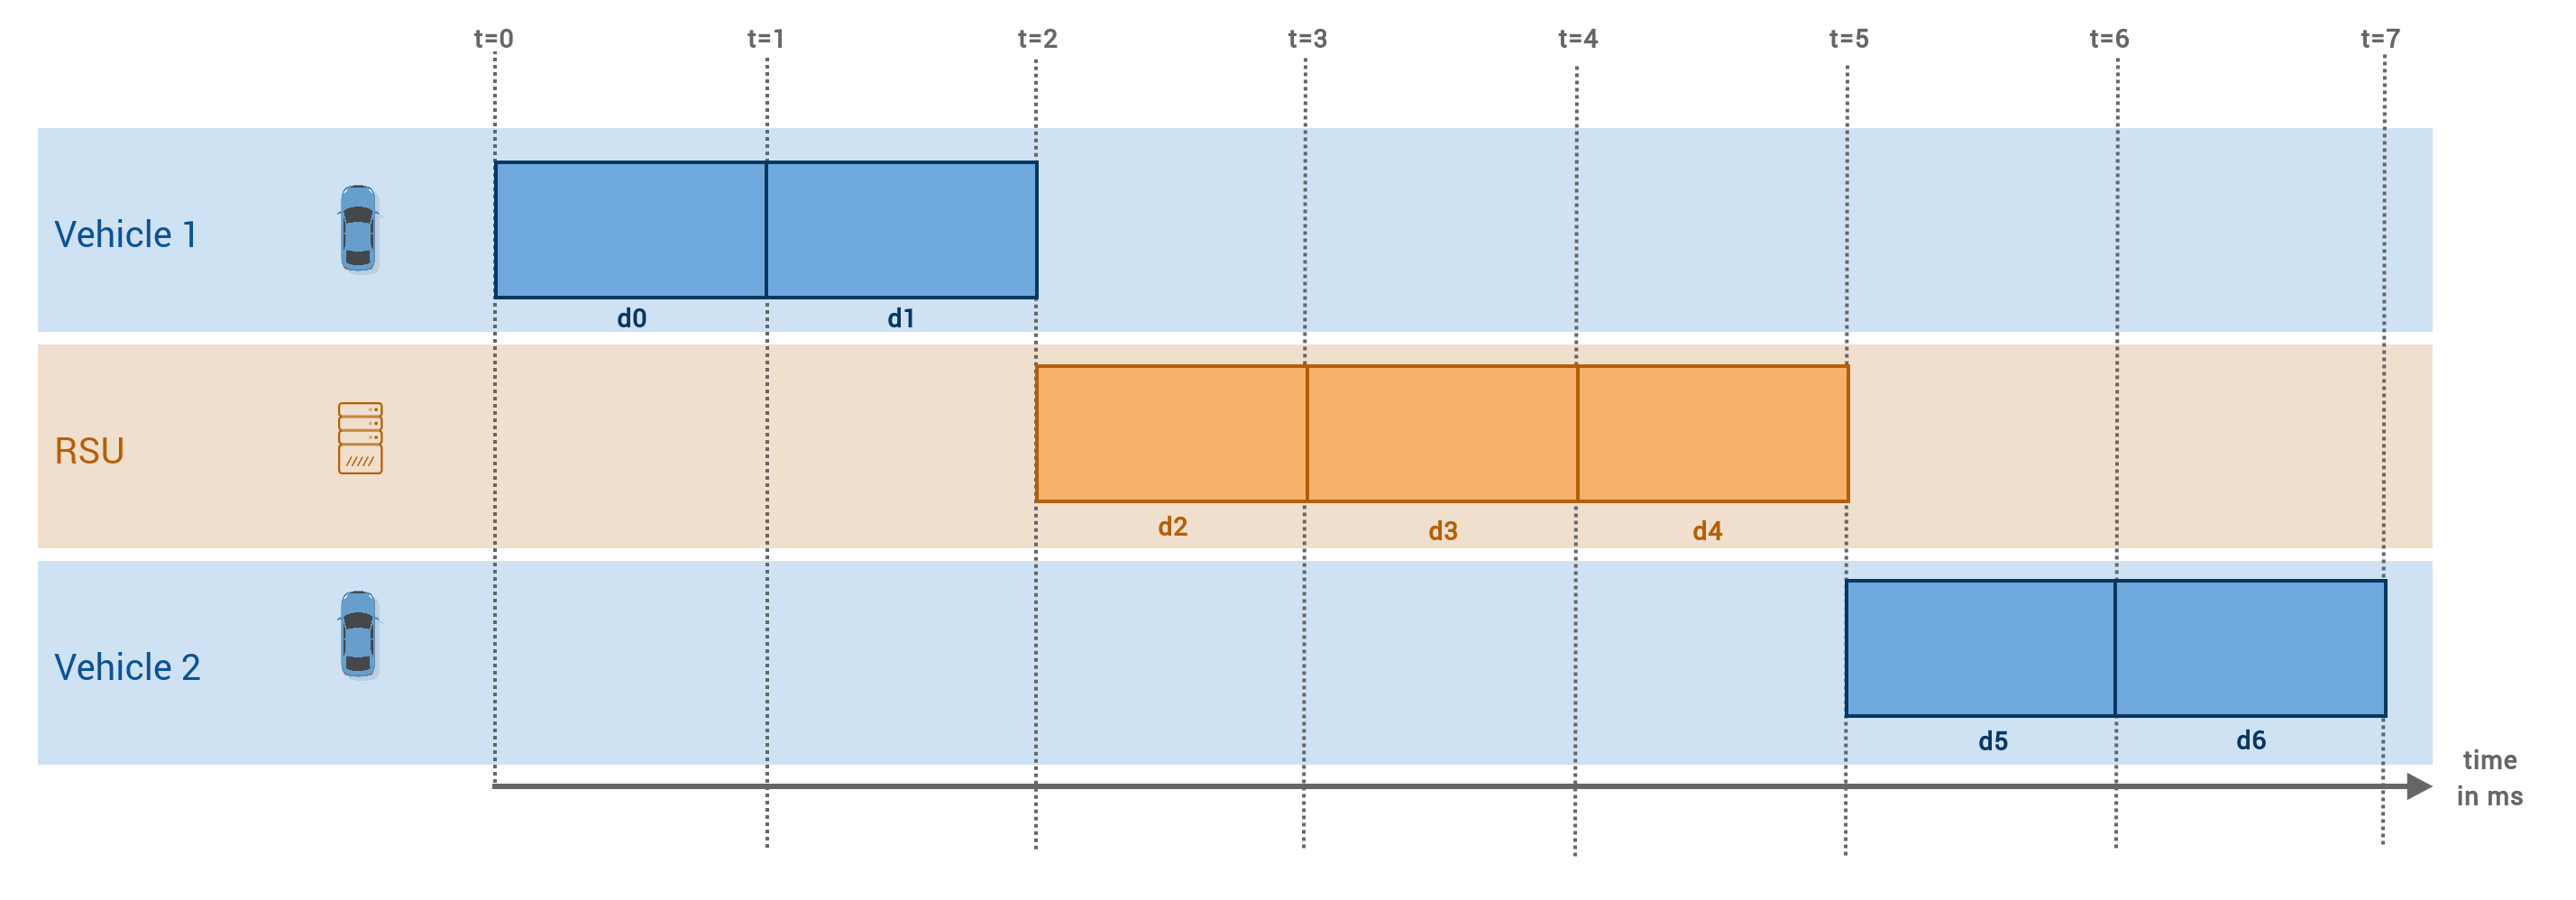
\includegraphics[width=1\linewidth]{98_images/communication_timeline}
	\caption{Timing Composition of Fusion Process}
	\label{fig:communication_timeline}
	\medskip
	\small
	\begin{enumerate}[t = 1:\ ]
		\item An observation is obtained by local sensory and low-level fusion (including ray casting-facilitated 5cell matching, etc., cf. \cref{subsec:implementation:talky_client}) \\
		\item The observation is encoded locally, i.e. represented as a PER model and serialized to Protobuf format
		\item The observation is received remotely, i.e. at the fusion node
		\item The observation is decoded remotely, i.e. deserialized from Protobuf and converted to process-local data structures
		\item The observation is remotely fused with other relevant observations from different observers, encoded to a PER model instance and serialized to Protobuf again
		\item The fused observation is received locally the ego vehicle
		\item The fused observation is decoded locally
	\end{enumerate}
\end{figure}

In order to gather (Q1), a minimalist sub-system of the entire CP software system is employed. It still follows a client-server architecture and has the message broker and fusion node on one end and multiple (simulated) ego vehicles on the other. Since we are only interested in quantitative measurements rather than in the messages' actual content, a newly created message generator program is used to artificially simulate observations instead of employing an actual Carla simulation with real Talky clients. Otherwise it would be infeasible to test with a large number of vehicles, due to exceedingly high computation load. The multi-threaded message generator is parameterized with (1) the target size of the generated occupancy grid observations, (2) the number of concurrent clients to simulate and (3) a per-client frequency at which to push messages to the backend (see \cref{tab:performance_evaluation:variable_parameters}). Moreover, supplementary code is added to the fusion node to track how often the \texttt{Publish()} method is called.

The test setup for (Q1) involves two physical machines, interconnected via a \SI{1}{\giga\bit\per\second} Ethernet network. One machine (AMD Ryzen 1600 \SI{3.2}{\giga\hertz} 6-core CPU, \SI{16}{\giga\byte} RAM, Ubuntu 18.04) runs the backend part of the system, i.e. message broker and edge node, while the message generator is run on the other (Intel i5-6600K \SI{4.5}{Ghz} 4-core CPU, \SI{16}{\giga\byte} RAM, Manjaro 18.1).
\par
\bigskip

\Cref{tab:performance_evaluation:constant_parameters} lists all fixed parameters used for the entire evaluation. Parameters marked with a star (*) are mentioned for completeness, but should not have any influence on the measured quantity. For the experiment, randomly generated occupancy grids lie within the same type 3 tile are used in the observation messages. \Cref{tab:performance_evaluation:variable_parameters} lists all variable, evaluation-specific parameters to be tested in order to get insights about their respective impact on the final results. To test all combinations of parameters for investigating (Q1), a grid search is conducted, i.e. a test is run for every combination in the Cartesian space of parameter values. For (Q2) and (Q3) only a single parameter set $\vartheta = \{ \texttt{N\_EGOS} = 6, \texttt{OBSERVATION\_RATE} = 10, \texttt{GRID\_RADIUS} = 11 \}$ is used.

\begin{table}
	\centering
	\begin{tabular}{|p{4.5cm}|p{2cm}|}
		\hline 
		\textbf{Parameter} & \textbf{Value} \\ \hline 
		\texttt{TILE\_1\_LEVEL} & \texttt{24} \\ \hline 
		\texttt{TILE\_2\_LEVEL} & \texttt{19} \\ \hline 
		\texttt{TILE\_3\_LEVEL} (*) & \texttt{15} \\ \hline 
		\texttt{MQTT\_QOS} & \texttt{1} \\ \hline 
		\texttt{DECAY\_FACTOR} (*) & \texttt{0.11} \\ \hline 
		\texttt{FUSION\_RATE} (*) & \texttt{10} \\ \hline 
		\texttt{OBSERVATION\_MAX\_AGE} & \texttt{3600} \\ \hline 
		\texttt{WITH\_OCCUPANT} & \texttt{false} \\ \hline 
	\end{tabular}
	\caption[Constant Parameters of the Performance Evaluation]{Constant Parameters of the Performance Evaluation. See \cref{sec:implementation:configurable_parameters} for descriptions.}
	\label{tab:performance_evaluation:constant_parameters}
\end{table}

\begin{table}
	\centering
	\begin{tabular}{|p{3.5cm}|p{8.5cm}|p{3.2cm}|}
		\hline 
		\textbf{Paremeter} & \textbf{Description} & \textbf{Values} \\ 
		\hline 
		\texttt{N\_EGOS} & Numbers of concurrent simulated clients exchanging CP messages & \texttt{\{25, 50, 75, 100, 200, 400, 800, 1600\}} \\ 
		\hline 
		\texttt{OBSERVATION\_RATE} & Frequency at which observations are periodically published to the network by each of its participants & \texttt{\{1, 5, 10\}} \\ 
		\hline 
		\texttt{GRID\_RADIUS} & Occupancy grid radius in number of cells. With $\lambda_1 = 24$ these are approx. equal to a grid size (i.e. observation range) of \texttt{\{52.8, 100.8\}} meters & \texttt{\{11, 21\}} \\ 
		\hline 
	\end{tabular}
	\caption{Variable Parameters of the Performance Evaluation}
	\label{tab:performance_evaluation:variable_parameters}
\end{table}

In summary, two steps are performed to gather the above metrics. First, to find (Q1), multiple iterations – each according to one parameter set – are run using the minimal system subset in the presented two-machine setup. Second, the entire CP system including a Carla simulation instance is run in a single machine to obtain (Q2) and (Q3) for a fixed parameter set. 

\subsection{Results}
\label{subsec:evaluation:performance_evaluation:results}
In accordance with the structure presented in the previous section, results are obtained in two steps.
\par
\bigskip

First, a set of experiments are conducted to get insights about the Talky edge node's \textbf{maximum fusion rate (Q1)}, depending on three different parameters. While most parameters, including the edge node's fusion rate, are fixed at a certain value (see \cref{tab:performance_evaluation:constant_parameters}), the number of concurrent network participants and their publishing frequency and grid size are varied. Consecutively executing the evaluation with a total of 30 different configurations yields the results depicted in \cref{fig:performance_evaluation:fusion_rates}.

\begin{figure}
	\centering
	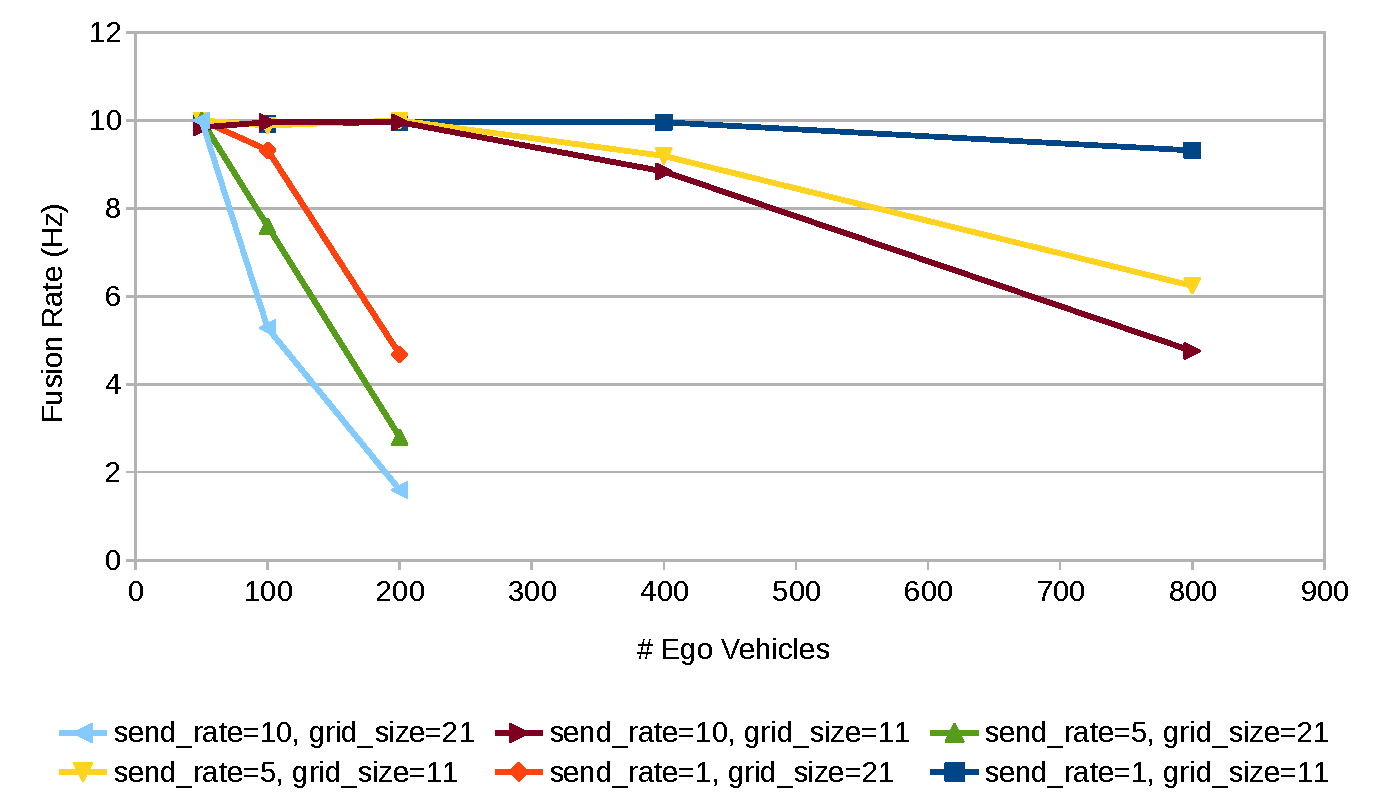
\includegraphics[width=1.0\linewidth]{98_images/performance_evaluation_chart1}
	\caption{Average Measured Fusion Rate}
	\label{fig:performance_evaluation:fusion_rates}
\end{figure}

It can be seen that the maximum possible fusion rate heavily depends on both the incoming message rate and the occupancy grids' size. While the fusion node is able to maintain a rate of \SI{10}{\hertz} for up to nearly 800 concurrent vehicles if their observation range is $\sim$ \SI{52.8}{\meter} (11 by 11 cells at $\lambda_1 = 24$), it tends to drop below that threshold as observation rate and grid size increase. Assuming a fusion rate of \SI{10}{\hertz}, the hard requirement of being able to handle $\sim$ 200 concurrent vehicles can only be fulfilled with the smaller observation range of \texttt{GRID\_RADIUS=11}, regardless of the client's publish frequency. If the client vehicles are expected to publish their environment observations from a range of $\sim$ \SI{100.8}{\meter} instead, the current Talky edge node implementation would not be able to keep up at a fusion rate of \SI{10}{\hertz}. However, if the system's fusion rate is lowered to, for instance, \SI{5}{\hertz} – which is still not an unrealistic value – the fusion node could fulfill the requirement for all test scenarios. As an additional excursus, the MQTT broker's performance is evaluated separately to eliminate the possibility of it constituting a bottleneck to the system. However, using the \texttt{mqtt-bench}\footnote{\url{https://github.com/takanorig/mqtt-bench}} benchmarking tool, it was found that Mosquitto (version 1.6.8) is able to handle up to \SI{8000}{messages\per\second} with a message size of \SI{12}{\kilo\byte} (approximately corresponding to 11x11-cell grids, see \cref{tab:performance_evaluation:message_sizes}) and up to \SI{4100}{messages\per\second} with a message size of \SI{46}{\kilo\byte} (21x21-cell grids). Therefore, the broker only becomes a limiting factor with more than 800 or 410 concurrent vehicles respectively. The benchmark results can be found in \cref{sec:appendix:evaluation_results:mqtt_broker_benchmark}.
\par
\bigskip

In a second step, average message size latency are investigated. Result for the former are depicted in \cref{tab:performance_evaluation:message_sizes}. The minimum achievable \textbf{average message size (Q2)} of a Protobuf-serialized PER model instance was found to be \SI{12}{\kilo\byte} (\SI{46}{\kilo\byte}) with a grid radius of 11 cells (21 cells), corresponding to an observation range $\sim$ \SI{52.8}{\meter} (\SI{100.8}{\meter}). Such minimalist message contains nothing but the observer information, the occupancy grid and an estimated state value for each cell. When including additional information on the occupant (vehicle, pedestrian, static obstacle, etc.) of a cell, the average message size increases accordingly.

\begin{table}
	\centering
	\begin{tabular}{|p{6.2cm}|p{3.5cm}|p{3.5cm}|}
		\hline 
		& \texttt{GRID\_RADIUS = 11} & \texttt{GRID\_RADIUS = 21} \\ 
		\hline 
		\texttt{WITH\_OCCUPANT = false} & \SI{12}{\kilo\byte} & \SI{46}{\kilo\byte} \\ 
		\hline 
		\texttt{WITH\_OCCUPANT = true} & \SI{32}{\kilo\byte} & 1\SI{21}{\kilo\byte} \\ 
		\hline 
	\end{tabular}
	\caption[Average Measured Observation Message Sizes]{Average  Measured Observation Message Sizes (occupied cells)}
	\label{tab:performance_evaluation:message_sizes}
\end{table}
\par
\bigskip

As a result of investigating how an observations total \textbf{latency (Q3)} is composed in the present CP system, the durations presented in \cref{tab:performance_evaluation:latency_composition} were observed. Instants and durations shown in the table refer to those presented in \cref{fig:communication_timeline}.

\todo{Write!}

\begin{table}
	\centering
	\begin{tabular}{|p{1.5cm}|p{5.1cm}|p{5.1cm}|p{1.8cm}|}
		\hline 
		Instant & Time Offset (with local perception) & Time Offset (without local perception) & Duration \\ 
		\hline 
		t=0 & 0 ms & – & – \\ 
		\hline 
		t=1 & 260 ms & 0 ms & 260 ms \\ 
		\hline 
		t=2 & 288 ms & 28 ms & 28 ms \\ 
		\hline 
		t=3 & 341 ms & 81 ms & 53 ms \\ 
		\hline 
		t=4 & 343 ms & 83 ms & 2 ms \\ 
		\hline 
		t=5 & 501 ms & 241 ms & 58 ms \\ 
		\hline 
		t=6 & 545 ms & 285 ms & 44 ms \\ 
		\hline 
		t=7 & 549 ms & 289 ms & 4 ms \\ 
		\hline 
	\end{tabular}
	\caption{Cooperative Perception Latency Composition}
	\label{tab:performance_evaluation:latency_composition}
\end{table}
\par
\bigskip

A further discussion about the implication of any of these results is done in the next section. 